%% ----------------------------------------------------------------------------
% BIWI SA/MA thesis template
%
% Created 09/29/2006 by Andreas Ess
% Extended 13/02/2009 by Jan Lesniak - jlesniak@vision.ee.ethz.ch
%% ----------------------------------------------------------------------------
\newpage
\chapter{Quantitative Analysis\label{sec:quantitative}}

\section{Selection}

4 volunteers were asked to annotate the wallpaper datasets.
For the Michael dataset, there is a correlation coefficient ($R$) of 0.49 in
annotations, while $R=0.28$ for the Wookie dataset.
It could already be seen that the Michael dataset is perhaps of higher quality
in terms of variety of objects imaged and lower repetitions.

When training a model on the Michael dataset and evaluating the model on the
Wookie dataset, there are 5 incorrect predictions for 135 images where
annotations agree.
This is an error rate of $3.7\%$, much lower than the opposite where training is
performed on the Wookie dataset and evaluation done on the Michael dataset.
In this case, there are 42 incorrect predictions for 141 images where
annotations agree.
This is a $29.8\%$ error, confirming that the quality of the Wookie dataset
could be improved.

Furthermore, we evaluate the performance of the classifier when training on
one's own annotations vs training on all available annotations.
While this error fluctuates for each annotator, the average error is $59.2\%$
for the case where training is performed using all available annotations.
This is a much higher error compared the case when training is only done using
an annotator’s own annotations ($29.2\%$ error).
An interesting study would be to see if combining annotations with high
correlation helps to improve the performance of the personalised classifier
of a user.

Another analysis done is the assessment of the Precision-Recall curve of the
classifiers (figure \ref{fig:PR}).
This is for the case when training on all annotations for either datasets and
evaluating on the other dataset.
For both cases, the trained models exhibit higher precision than the case where a random classifier is used.
The decision function of a random classifier returns a uniformly distributed random number in the range of expected values.
It can therefore be concluded that the classifiers serve their purposes.
In the case of the model trained on the Wookie set however, the base precision of $0.4$ is quite high, indicating that the annotations may not be well balanced.

\begin{figure}
\centering
\begin{subfigure}{0.79\columnwidth}
  \centering
  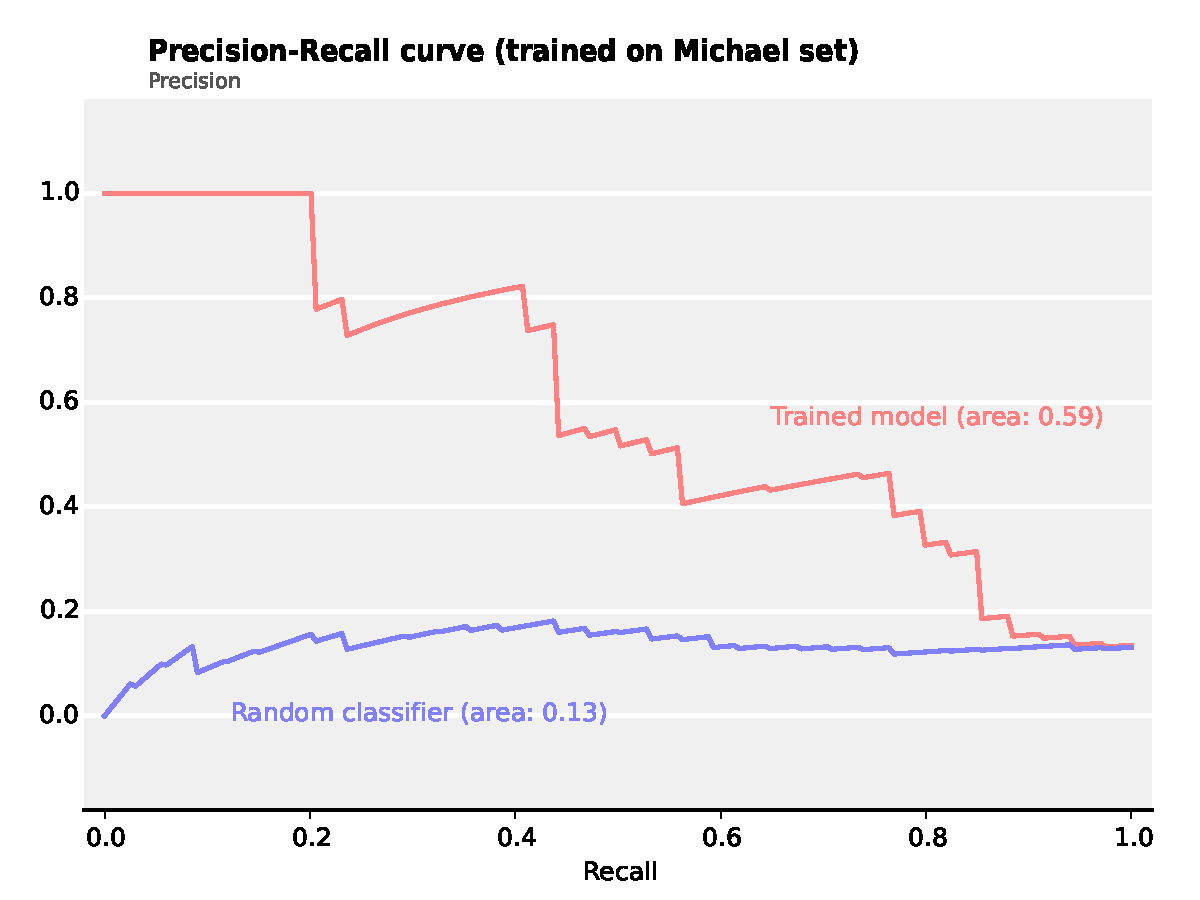
\includegraphics[width=0.99\columnwidth]{../figures/PRcurve_michael_wookie.pdf}
  \caption{Classifier trained on Michael set, evaluated on Wookie set.}
\end{subfigure}
\vskip8mm
\begin{subfigure}{0.79\columnwidth}
  \centering
  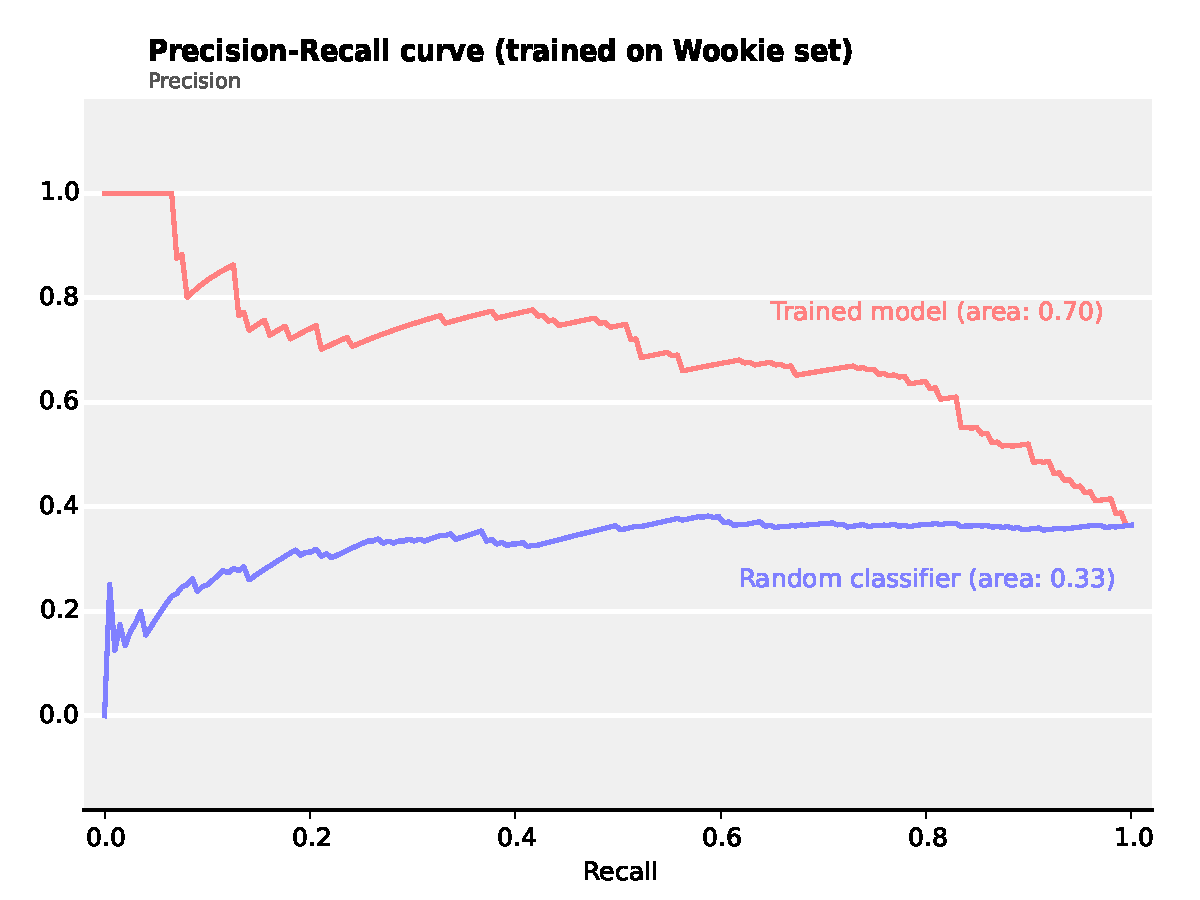
\includegraphics[width=0.99\columnwidth]{../figures/PRcurve_wookie_michael.pdf}
  \caption{Classifier trained on Wookie set, evaluated on Michael set.}
\end{subfigure}
\caption{Precision-Recall curve plots for trained wallpaper suitability models.\label{fig:PR}}
\end{figure}


\newpage
\section{Cropping\label{sec:quant_cropping}}

As mentioned in section \ref{sec:method_cropping}, the proposed algorithm is built on that suggested in \cite{fang2014automatic}.
The differences are:

\begin{enumerate}
\item 4 separate boundary features used in training as opposed to a single
      boundary simplicity score post-classification.
\item A shrinking crop size algorithm for candidate crop generation.
\item The use of a Reddit-based dataset for training.
\end{enumerate}

To evaluate the effect of these changes quantitatively, the evaluation method
introduced in \cite{fang2014automatic} is used.
This starts with the use of a 500-image dataset annotated with the use of Amazon Mechanical Turk.
Each image has 10 associated ideal crop which can be regarded as a ground truth crop.
This human crop dataset is used for quantitative evaluation.

Given a candidate crop $C_i$, the maximum overlap between the crop and available
human crops is calculated as shown in equations \ref{eq:Overlap} and \ref{eq:MaxOverlap}.
This can be assessed for just the top crop candidate as well as up to top 5 crop
candidates.
It is expected that the maximum overlap increases with more top candidates
considered as the model is not perfect and the true top crop candidate may be a
few places offset.

\begin{align}
	\mathrm{Overlap}(C_i, H_j)  &= \frac{C_i \cap H_j}{C_i \cup H_j} \label{eq:Overlap}\\
	\mathrm{MaxOverlap}(C_i, H) &= \max_j\mathrm{Overlap}(C_i, H_j)  \label{eq:MaxOverlap}
\end{align}

The maximum overlap scores over top 5 crop candidates is calculated over the
mentioned 500-image dataset to yield scores as seen in figure \ref{fig:cropping_comparison}.
It can be seen that the suggested algorithm works better in general.
The standard error of maximum overlap values are negligible and therefore it can
be seen that the proposed implementation is an improvement over \cite{fang2014automatic}.
Consequently, compared to \cite{park2012modeling} and \cite{yan2013learning} the
top 1 candidate score is a marked improvement.
Compared to \cite{yan2013learning}, our method is almost a 2x improvement.
It should also be noted that the maximum overlap score increases slower for our
method than compared to earlier methods.
This indicates that the top crop candidates are more reliable.

In terms of \textrm{MaxOverlap} values, our implementation yields $0.782\pm0.004$
when top 1 crops are considered with the value increasing up to $0.860\pm0.003$
for the case of top 5 crops being considered.

\begin{figure}
\centering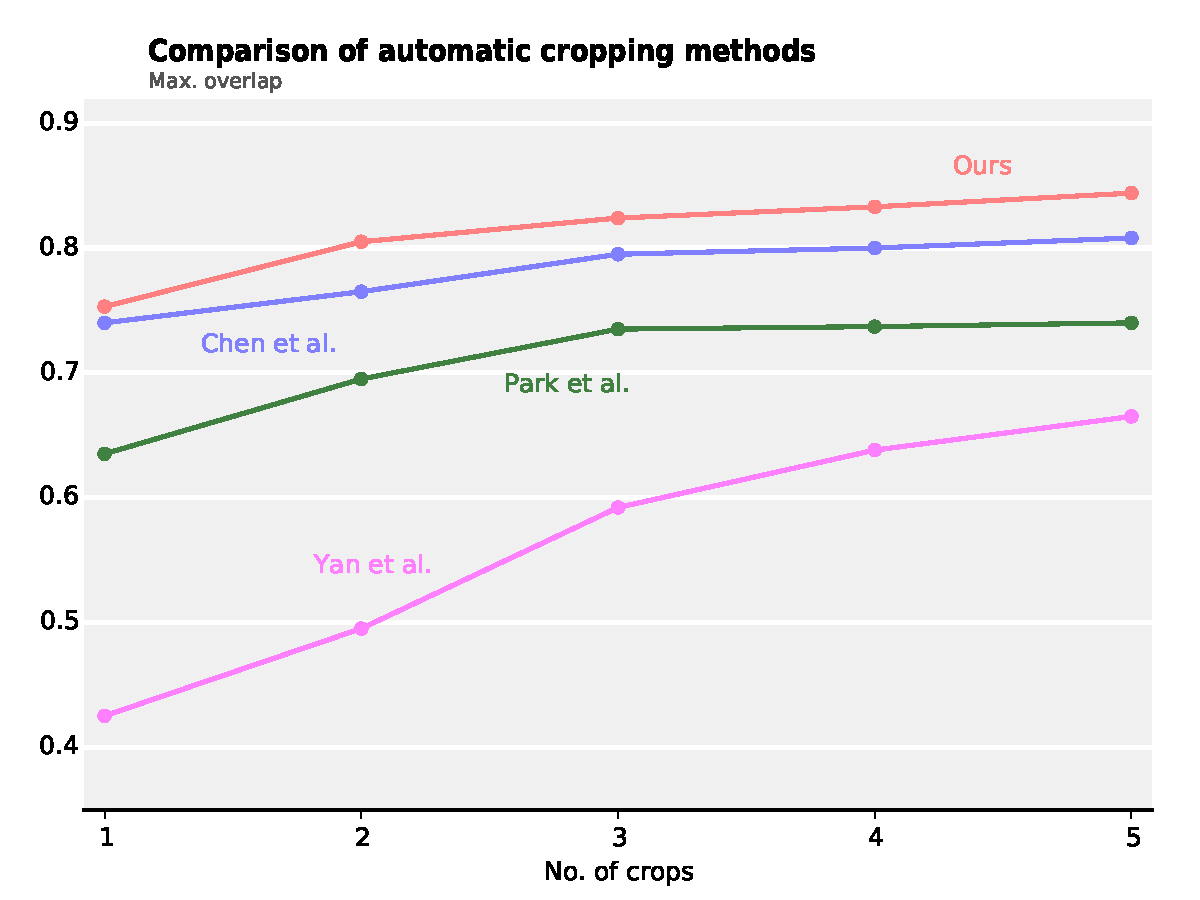
\includegraphics[width=\columnwidth]{../figures/comparison.pdf}
\caption{Quantitative evaluation of various automatic cropping algorithms
	\cite{fang2014automatic,park2012modeling,yan2013learning}.\label{fig:cropping_comparison}}
\end{figure}

